\section{Theorie}
\label{sec:Theorie}
Ein Lock-In-Verstärker besteht prinzipiell aus einem Bandpassfilter, einem Signalmischer und einem Tiefpassfilter, wie es schematisch in \autoref{fig:schema} dargestellt ist. Der Bandpassfilter befreit das verrauschte Nutzsignal $U_\text{sig}$ von den hoch- und niedrigfrequenten Anteilen. Im Mischer wird das Nutzsignal dann mit einem Referenzsignal $U_\text{ref}$ mit der Frequenz $\omega_0$ multipliziert. Hinter dem Mischer ist ein Tiefpass ($\tau = RC ≫ 1/\omega_0$) verschaltet,  der das Mischsignal  $U_\text{sig} \times U_\text{ref}$ integriert. Mit einem solchen Lock-In-Verstärker sind Güten in einem Bereich von $Q=100000$ erreichbar, während eine reine Bandpass-Schaltung nur Güten in einem Bereich von $Q=1000$ erreicht.
\begin{figure}[H]
    \centering
    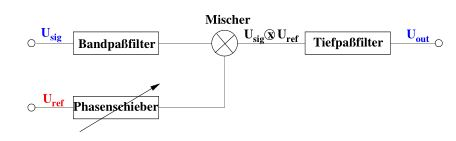
\includegraphics{images/schema.JPG}
    \caption{Schematischer Aufbau eines Lock-In-Verstärkers\cite{sample}}
    \label{fig:schema}
\end{figure}
\noindent
Im Folgenden werden die Signal- und die Referenzspannung mathematisch betrachet.
Für die Signalspannung wird ein sinusförmiger Verlauf nach  

\begin{equation}
    U_\text{sig} = U_0 \cdot \sin(\omega \cdot t)
    \label{eqn:usig}
\end{equation}
\noindent
angenommen.
Die rechteckige Referenzspannung kann durch eine Fourierreihe, die sich aus den ungeraden Harmonischen der Grundfrequenz $\omega$ zusammensetzt, nach \autoref{eqn:uref} angenähert werden:

\begin{equation}
    U_\text{ref} = \frac{4}{\pi}(\sin(\omega \cdot t) + \frac{1}{3}\sin(3\omega \cdot t) +  \frac{1}{5}\sin(5\omega \cdot t) + ...)
    \label{eqn:uref}
\end{equation}
\noindent

Im Mischer werden diese beiden Signale multipliziert, sodass sich das Signal 

\begin{equation}
    U_\text{sig} \times U_\text{ref} = \frac{2}{\pi} \cdot U_0(1 - \frac{2}{3}\cos(2\omega \cdot t)  -  \frac{2}{15}\cos(4\omega \cdot t) - \frac{2}{35}\cos(6\omega \cdot t)...)
    \label{eqn:urefsig}
\end{equation}
\noindent
ergibt. Im nachgeschalteten Tiefpass werden nun die Oberwellen des gemischten Signals unterdrückt. So entsteht eine Ausgangsspannung, die proportional zur Signalspannung ist:
\begin{equation}
    U_\text{out} = \frac{2}{\pi} U_0 
    \label{eqn:uout}
\end{equation}
\noindent
Wenn eine Phasendifferenz $\phi$ zwischen Signal- und Referenzspannung besteht, erhält man in \autoref{eqn:uout} zusätzlich einen Faktor für die Phase:
\begin{equation}
    U_\text{out} = \frac{2}{\pi} U_0 \cdot \cos(\phi)
    \label{eqn:uout2}
\end{equation}
\noindent
Die Ausgangsspannung wird also für eine Phase von $\phi=0$ maximal.